\chapter{Výběr a návrh elektroniky}

\section{Bezdrátová technologie}
Ke komunikaci Semaforů mezi sebou byla zvolena technologie LoRa. Tato technologie byla zvolena především kvůli komunikačnímu dosahu. Jedná se sice o dražší technologii, 
ale na tolik, aby ji nebylo možné v tomto zařízení použít. Táborové hry se většinou hrají na loukách, které mají rozlohu několik stovek metrů čtverečných. LoRa je jedinou
dostupnou technologií, která na tyto vzdálenosti spolehlivě komunikuje. Bezdrátové propojení Semaforů bude použito pro posílání informací o aktuálně svítící barvě, či 
stisku tlačítka v závislosti na hře, která se aktuálně hraje. U některých her například může být žádoucí, aby po přepínání nesvítily všechny Semafory stejnou barvou,
díky této komunikaci se bude moci být takovým stavům zabráněno. 

K propojení Semaforu s telefonem a dalšími zařízeními byla vybrána technologie WiFi. Jedná se o rozšířenou technologii, která je v telefonech a noteboocích zabudovaná. 
Propojení bude tedy jednoduché a nastavovat hry se mohou na webové stránce. Mikrokontrolér vytvoří WiFi, ke které se pomocí telefonu připojí. Po připojení bude zobrazena
webová stránka, kde bude seznam her, které Semafor umí. U jednotlivých her se poté budou moci nastavovat další parametry. Po nasatvení se komfigurace pošle do Semaforu. 

\section{Mikrokontrolér}
WiFi modul obsahuje jako jediný mikrokontrolér od firmy Espressif z řady ESP32. Konkrétně jde o typ ESP32-C3-MINI, dále již je ESP32-C3. Je také nabízen za cenu, která 
je v porovnání s ostatními nízká a v porovnání s nabízenými parametry bezkonkurenční. Pro zařízení Semaforu je také se svým počtem periferií dostačující. ESP32-C3 má 
384 kB ROM a 4 MB flash paměti \cite{ESP_C3_dtsh}. Dále obsahuje WiFi modul pracující na frekvenci 2,4 GHz a Bluetooth \cite{ESP_C3_dtsh}. ESP32-C3 obsahuje SPI, UART, 
$I^2C$, USB a další \cite{ESP_C3_dtsh}. V mikrokontroléru je také zabudován krystal s vlastní frekvencí 40 MHz a v rámci pouzdra je také anténa pro WiFi \cite{ESP_C3_dtsh}.

Rozsah napájecího napětí je 3 až 3,6 V \cite{ESP_C3_dtsh}. Jeho průměrný proudový odběr je XXX a jeho minimální odběr proudu v režimu spánku je XXX %dopsat
Mikrokontrolér ESP32-C3 garantuje pracovní teplotu od -45 °C až do 85 °C \cite{ESP_C3_dtsh}.

%napsat o strapping pins

Mikrokontrolér ESP32-C3 nemá kapacitní vstupy a proto je zapotřebí pro kapacitní tlačítka použít převodník pro zpracování signálu z nich \cite{ESP_C3_dtsh}. 

%schéma zapojení a připojení všech periferií

\section{LED}
Jedním z nejdůležitějších požadavků na Semafor bylo, aby mohl svítit. Čím více možností, jak svítit, tím bude využití 
při hrách a táborových programech různorodější. K tomuto účelu jsou použity LED. 

K tomu by byl zapotřebí mikrokonrolér s velkým množství GPIO pinů. Takových mikrokonrolérů není mnoho a zároveň 
by se to odrazilo na ceně. Počet GPIO pinů je jedním z hlavních limitujících faktorů při výběru MCU. Proto byly použity programovatelné 
LED typu WS2812C.

\begin{figure}[!h]
  \begin{center}
    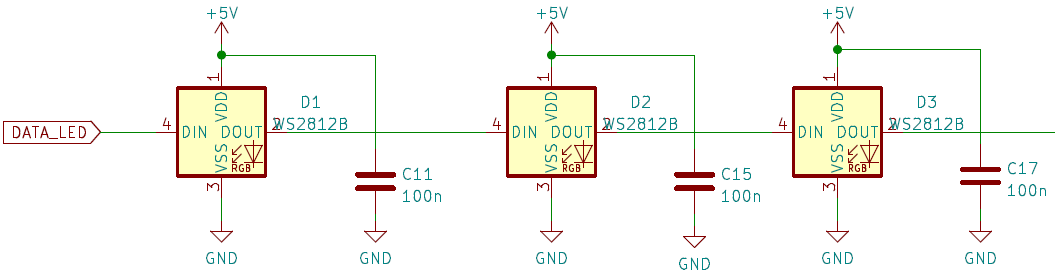
\includegraphics[scale=0.5]{obrazky/WS2812C.png}
  \end{center}
  \caption[Zapojení inteligentních LED WS2812C]{Zapojení inteligentních LED WS2812C.}
\end{figure}

Komunikační napěťová úroveň logické jedničky těchto LED by měla být alespoň na úrovni 70 \% napájecího napětí \cite{WS2812C_dtsh}. 
Protože použitý mikrokonrolér ESP32-C3 má komunikační napěťovou úroveň logické jedničky jeho napájecí napětí, což je 3 až 3,6 V, 
tak je zapotřebí využít převodník napěťové úrovně \cite{ESP_C3_dtsh}. Komunikace je v tomto případě pouze jednosměrná, 
to znamená, že MCU posílá data do LED, ale LED neposílají žádná data do MCU. Převodník je realizován unipolárním tranzistorem 
a jedním pullup rezistorem. Rezistor je připojen pro k napájecímu napětí inteligentních LED WS2812C. 
Tranzistor Q1 má gate připojený k napájecímu napětí MCU. Pokud bude mikrokonrolér do LED posílat logickou jedničku, tak bude rozdíl
mezi gate a source 0 V. Tím pádem bude tranzistor uzavřený a tím se přes rezistor R4 připojí k LED jejich napájecí napětí. Toto napětí 
je pro inteligentní LED logickou jedničkou. Pokud bude MCU posílat logickou nulu, tedy 0 V, tak je rozdíl napětí mezi gate a source 
napájecí napětí mikrokontroléru. Tranzistor je tedy otevřený a tím se napětí 0 V dostane k inteligentním LED a na rezistoru se objeví
úbytek napětí o velikosti napájecího napětí inteligentních LED. Napětí 0 V je logickou nulou i pro inteligentní LED. Tento převodník
je určen pouze pro komunikaci jedním směrem. 

\begin{figure}[!h]
  \begin{center}
    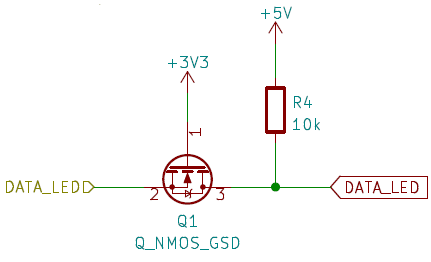
\includegraphics[scale=0.6]{obrazky/prevodnik_urovni_pro_WS2812C.png}
  \end{center}
  \caption[Zapojení převodníku úrovní pro WS2812C]{Zapojení převodníku úrovní pro WS2812C.}
\end{figure} 

Tyto programovatelné LED mají maximální spotřebu 5 mA na jeden kanál. Při zapnutí všech kanálů (svícení bílou) je maximální
spotřeba jedné LED 15 mA \cite{WS2812C_dtsh}. Pokud LED nesvítí, tak je její maximální klidový proud 0,3 mA \cite{WS2812C_dtsh}.
Při použití 12 LED je tedy maximální odběr všech LED 180 mA.

Kondenzátor u každé LED slouží pro filtraci napájecího napětí. 

\section{Vibrační motor}
Vibrační motory jsou založeny na principu kmitání. Motor je připevněn k zařízení, které je kmitáním rozvibrováno. Vibrační motory jsou dnes 
nedílnou součástí mnoha elektronických zařízení včetně mobilního telefonu nebo dětských hraček. 

Dioda slouží jako ochrana proti přepětí, protože motor je indukční zátěž, takže vytváří napěťové špičky. Díky diodě je mikrokonrolér chráněn 
proti špičkovému napětí, které by se na něj mohlo dostat. Kondenzátor slouží k tomu, aby napěťové špičky eliminovat, nebo alespoň zmenšoval. 

Vibrační motor je připojen k mikrokontroléru přes tranzistor, protože maximální výstupní proud z pinu MCU není dostatečně velký na to, aby 
motor roztočil. Tranzistor je tedy připojen na gate tranzistoru, který se při logické jedničce na pinu sepne a motorem protéká proud, který 
nedodává MCU, ale zdroj 3.3 V (v tomto případě baterie LiFePO4). Baterie tak dokáže dodat dostatek proudu, aby se motor roztočil. 

Pro Semafor byl vybrán vibrační motor LCM1020A2945F. Tento motor má maximální požadovaný proud 120 mA \cite{vib_motor_dtsh}. Maximální proud, 
který lze odebírat z pinu mikrokontroléru ESP32-C3, je 40 mA \cite{ESP_C3_dtsh}. Vibrační motor lze pouze spínat, nebo je možné jej připojit 
k pinu, který dokáže generovat PWM a lze tím regulovat jeho otáčky. 

Vibrační motor slouží jako odezva na dotyk kapacitního tlačítka. 

%obrázek schéma zapojení + asi fotka vybraného motoru

\section{Převodník pro kapacitní tlačítka}
%převodník AT42QT1070
Jelikož je v tomto návrhu Semaforu využit mikrokontrolér, který podporuje komunikaci po sběrnici I2C, tak bylo využito právě zapojení s komunikací 
přes I2C. Díky tomu budou využity pouze 2 GPIO piny mikrokonroléru ESP32-C3 a ne 5 GPIO pinů, které by byly zapotřebí při zapojení bez komunikace pro
sběrnici I2C.

Převodník má kondenzátory C3 a C4 připojeny na napájecím pinu vůči zemi, aby nebyly případné proudové špičky přivedeny na napájení převodníku. Rezistory
R17 a R18 slouží jako pullup rezistory při komunikaci pomocí sběrnice I2C s mikrokonrolérem EP32-C3. Na piny KEY0 až KEY4 jsou připojena kapacitní 
dotyková tlačítka.  
%proč je MODE na zemi
%proč nepoužívám pin /CHANGE?

\begin{figure}[!h]
    \begin{center}
      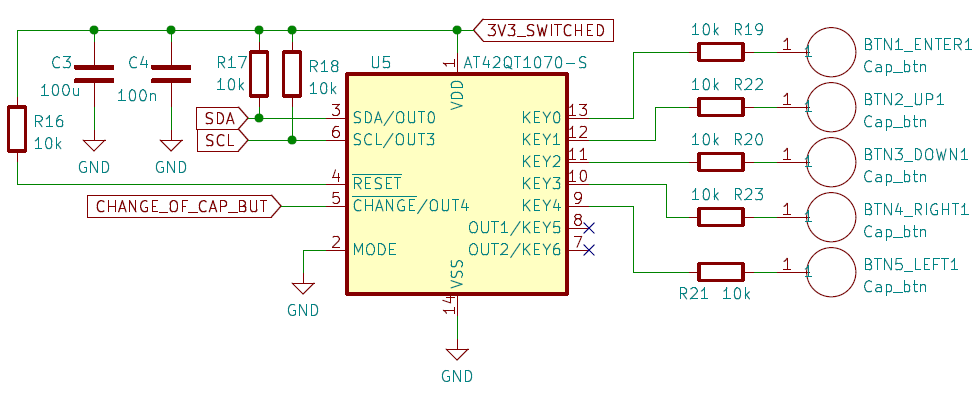
\includegraphics[scale=0.4]{obrazky/AT42QT1070.png}
    \end{center}
    \caption[Zapojení převodníku AT42QT1070 pro kapacitní tlačítka]{Zapojení převodníku AT42QT1070 pro kapacitní tlačítka.}
\end{figure}

\section{Napájení}
Při realizaci Semaforu byl vybrán článek baterie LiFePO4 právě kvůli již zmíněným vynikajícím vlastnostem. Vybraný mikrokonrolér má napájecí napětí v rozsahu 3 až 3,6 V \cite{ESP_C3_dtsh}. 
Pro funkci mikrokontroléru tedy nebude muset být použit ani převodník napětí.  


\subsection{Nabíjecí obvod}
%nastavit nabíjecí proud na 1C 
Nabíjecí obvody jsou závislé na konkrétním typu baterií, které budou nabíjeny. Vzhledem k vybranému typu baterií LiFePO4 byly uvažovány pouze komerčně
dostupné integrované obvody, které jsou určeny pro nabíjení tohoto typu baterií. 
%ještě TP5000 zmínit? - zkontrolovat jestli je opravdu na pro LiFePO4

Vybraný typ baterií LiFePO4 lze nabíjet pomocí obvodu CN3058E \cite{charger_dtsh}. 
%možná vyjmenovat další obvody a napsat proč tento

%napětí nastaveno na 3,6 V interně, ale lze jej nastavit pomocí externího odporu
%nabíjecí proud se nastavuje externím rezistorem - není využito
%při odpojení napájecího napětí přechází tento obvod do režimu spánku, takže je baterie vybíjena proudem menším než 3 uA
%lze snímat teplotu na baterii

Nabíjecí obvod CN3058E je určen pro nabíjení pouze LiFePO4 baterií a lze jím napájet právě 1 článek těchto baterií \cite{charger_dtsh}. Napájecí napětí tohoto 
nabíjecího čipu se pohybuje mezi 3,8 až 6 V \cite{charger_dtsh}. Díky tomu lze přímo použít napětí z USB konektoru. 

%popsat další vlastnosti 

%doporučené schéma zapojení čipu - z datasheetu

Tento nabíjecí obvod se vyrábí ve standardizovaném pouzdře SOP8 \cite{charger_dtsh}.

\subsection{Zapojení nabíjecího obvodu}
Rezistor připojený k pinu ISET slouží pro nastavení hodnoty nabíjecího proudu \cite{charger_dtsh}. V tomto zapojení byl počítán pro nabíjecí proud 1 A dle rovnice: 
\begin{equation} 
  I_{CH}~=~\frac{U_{ISET}}{R_{8}}~\cdot~1011. 
  \quad \quad \quad \quad \quad \quad \cite{charger_dtsh}
\label{eq:I_CH}
\end{equation}

%1218/1 = 1218 Ohm
%rovnici + citace


%jak zjistim napeti na tom pinu?
Velikost rezistoru R8 byla počítána na velikost nabíjecího proudu 1 A dle následující rovnice:
\begin{equation} 
  R_{8}~=~\frac{U_{ISET}}{I_{CH}}~\cdot~1011~=~\frac{}{1}~\cdot~1011~=~XXX~\:k\Omega. 
  \quad \quad \quad \quad \quad \quad \cite{charger_dtsh}
\label{eq:R_8}
\end{equation}


%tuto větu opravit
Z výpočtu vyplývá, že rezistor by měl mít hodnotu 1218 $\Omega$. Nejbližší hodnota z rezistorové řady E12 je hodnota 1,2 k$\Omega$, proto byl také zvolen rezistor 
o této hodnotě \cite{rezistorova_rada}. Odpovídá tomu nabíjecí proud 1015 mA, který nebude mít vliv na životnost baterií. 

%rovnice 1218/1200 = 1.015 A = 1015 mA

Vstupní a výstupní kondenzátory slouží pro filtaci zákmitů napájecího napětí a také napětí, kterým je nabíjena baterie. Hodnoty kondenzátorů byly převzaty
z doporučení z datasheetu.

Kladný pól nabíjené baterie je připojen na pinu BAT, záporný pól je připojen ke GND. Pin BAT poskytuje nabíjecí proud do baterie a zároveň poskytuje konstantní 
nabíjecí napětí. V režimu spánku je svodový proud tohoto pinu 3 $\mu$A \cite{charger_dtsh}. 

Pin VIN slouží pro napájení vnitřního obvodu CN3058E. Je na něj přikládáno napájecí napětí z USB, tedy 5 V. Pokud napájecí napětí klesne na napětí o 10 mV nižší, 
než je napětí na pinu BAT, tak vnitřní obvod přechází do režimu spánku \cite{charger_dtsh}. V tomto režimu klesá proud pinu BAT na méně než 3 $\mu$A \cite{charger_dtsh}.

Tento nabíjecí obvod má možnost indikace nabíjení baterií a dokončení nabíjení. Tato indikace je realizována pomocí 2 LED připojených přes pullup rezistor. Hodnota
pullup rezistoru byla převzata z doporučení z datasheetu. Červená LED indikuje nabíjení baterií a je připojena na pin /CHRG a zelená LED indikuje dokončené nabíjení 
a je připojena na pin /DONE. Obě LED jsou k pinům nabíjecího čipu připojeny katodou. 

Obvod CN3058E může také měřit teplotu na nabíjené baterii. Slouží k tomu vstupní pin TEMP. Měření probíhá pomocí odporového děliče, jehož střed je připojen na snímač 
teploty. Tento snímač je připojen na baterii. Pokud je napětí na pinu TEMP nižší než 45 \% nebo vyšší než 80 \% úrovně napájecího napětí, tak je indikována moc nízká
nebo moc vysoká teplota baterie a nabíjení je zastaveno \cite{charger_dtsh}. Jinak nabíjení pokračuje. Uzemněním pinu TEMP je funkce měření teploty deaktivována \cite{charger_dtsh}. 
V této práci není měření teploty baterií využíváno, a proto je pin TEMP připojen ke GND. 

%obrázek z datasheetu, kde je připojeno i meření teploty

Pokud není baterie nabíjena, tak by svodový proud pinu BAT nabíjecího obvodu CN3058E vybíjel baterii. Svodový proud tohoto pinu je 3 $\mu$A \cite{charger_dtsh}. 
Aby se baterie zbytečné navybíjela, tak je do obvodu připojen tranzistor Q2, který detekuje připojené napětí k nabíjecímu obvodu. Pokud je napětí připojeno, tak je 
tranzistor otevřen a baterie je nabíjena. Pokud napětí připojeno není, tak je tranzistor uzavřen a baterie je díky tomu odpojena od nabíjecího obodu. Díky tomu 
není vybíjena svodovým proudem pinu BAT. 

\section{Zvyšovač napětí pro LED}
Pro napájení vybraných inteligentních LED je zapotřebí napětí v rozsahu 4,5 až 5,5 V \cite{WS2812C_dtsh}. Použité baterie LiFePO4 mají napětí pouze 3,2 V, proto je 
zapotřebí použít zvyšovač napětí. 

Z komerčně dostupných integrovaných obvodů byl hledán zvyšovač napětí, který vytváří z napětí 3,3 V napětí 5 V a dodávat přitom do výstupu proud alespoň 200 mA. 
Maximální odběr všech 12ti potřebných inteligentní LED má maximální odběr 180 mA. S rezervou je tedy zapotřebí proud alespoň 200 mA. Nalezené obvody, které vyhovují 
těmto parametrům jsou LT1930 a MCP1640. 

Obvod LT1930 v doporučeném zapojení při vstupním napětí 3,3V vytváří výstupní napětí o hodnotě 5 V s maximálním odběrem proudu 480 mA \cite{LT1930_dtsh}. Napájecí napětí 
tohoto obvodu je v rozsahu 2,45 V až 16 V, což vyhovuje napájecímu napětí z baterií LiFePO4 \cite{LT1930_dtsh}.

%krátký popis MCP1640

%proč byl vybrán právě tento?
%Pro realizaci Semaforu byl zvolen obvod LT1930, který XXX protože XXX
%schéma zapojení vybraného typu

Pin /SHDN slouží k zapínání a vypínání obvodu. Pomocí přiloženého napětí 2,4 V a více na tento pin je obvod zapnut \cite{LT1930_dtsh}. Pin SW slouží pro  připojení cívky, 
případně diody, aby se snížilo elektromagnetické rušení \cite{LT1930_dtsh}. 

Pin FB slouží  pro zapojení zpětné vazby napětí na baterii. Jeho referenční napětí musí být nastaveno v rozmezí 1,240 V až 1,270 V, typická hodnota je však 1,255 V \cite{LT1930_dtsh}. 
Pro výstupní napětí 5 V byl zvolen rezistor R10 o hodnotě 13 k$\Omega$ z rezistorové řady E24 \cite{rezistorova_rada}. Řada E24 byla zvolena kvůli požadované přesnosti
napětí na pinu FB obvodu LT1930. Napětí na rezistoru R10 musí být tedy 1.255 V. Na rezistoru R9 je tedy úbytek napětí 3,745 V. Pomocí trojčlenky byla dopočítána hodnota 
rezistoru R9 dle rovnice:
\begin{equation} 
  R_{9}~=~\frac{R_{10}~\cdot~U_{R9}}{U_{R10}}~=~\frac{13~\cdot~3,745}{1,255}~=~38,79~\:k\Omega. 
  \quad
\label{eq:R9}
\end{equation}

Nejbližší hodnota rezistoru z rezistorové řady E24 je 39 k$\Omega$ \cite{rezistorova_rada}. Reálná hodnota napětí na rezistoru R10, tj. napětí na pinu FB byla dopočítána
dle rovnice:
\begin{equation} 
  U_{R10}~=~\frac{U_{OUT}}{R_{9}~+~R_{10}}~\cdot~R_{10}~=~\frac{5}{39~+~13}~\cdot~13~=~1,25~V. 
  \quad
\label{eq:UR10}
\end{equation}

Napětí 1,25 V je v povoleném rozmezí napětí na pinu FB. 

Přesné výstupní napětí se spočítá podle vzorce:
\begin{equation} 
  U_{OUT}~=~U_{FB}~\cdot~(1~+~\frac{R_{9}}{R_{10}})~=~1,25~\cdot~(1~+~\frac{39}{13})~=~5~V. 
  \quad \quad \quad \quad \cite{LT1930_dtsh}
\label{eq:VOUT_LT1930}
\end{equation}

%výběr diody
%výběr cívky

\begin{figure}[!h]
  \begin{center}
    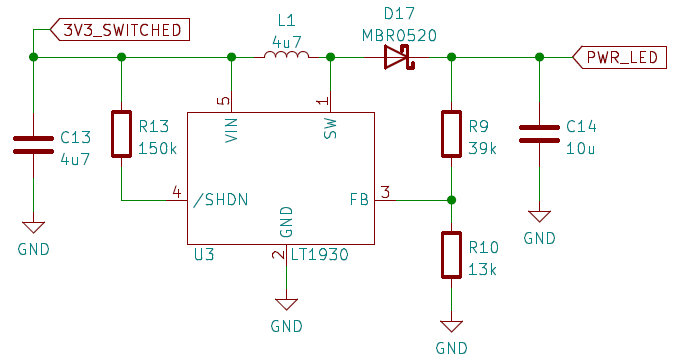
\includegraphics[scale=0.7]{obrazky/LT1930.png}
  \end{center}
  \caption[Zapojení zvyšovače napětí LT1930]{Zapojení zvyšovače napětí LT1930.}
\end{figure}

\section{Konektor}
Jako programovací konektor byl zvolen konektor USB typu C, který může být použit i jako konektor pro nabíjení baterie.

Tento konektor je v dnešní době velmi rozšířený a jeho použití se v následující době stále rozšiřuje. 

Není využíváno žádných výhod konektoru USB-C, jako je např. možnost power delivery apod. Je využíván pouze jako standardní a dostupný konektor, který je mezi běžnou
populací rozšířený a v následujících letech se bude rozšiřovat stále více. Je využito standardního jmenovitého napětí 5 V pro nabíjení baterií a nadále pinů D+ a D-, 
které jsou využity pro komunikaci při programování. 

Konektor USB-C je robustní a oboustranný, díky čemuž nebude docházet k tak častému poškození, jak by mohlo být např. u konektoru Micro USB. Při používání běžnou veřejností
se jedná o vítaný bonus. 

Vybraný mikrokonrolér ESP32-C3 umožňuje komunikaci přímo po USB protokolu a není díky tomu zapotřebí žádného převodníku pro komunikaci \cite{ESP_C3_dtsh}. %jmenuje se to USB protokol?

\begin{figure}[!h]
  \begin{center}
    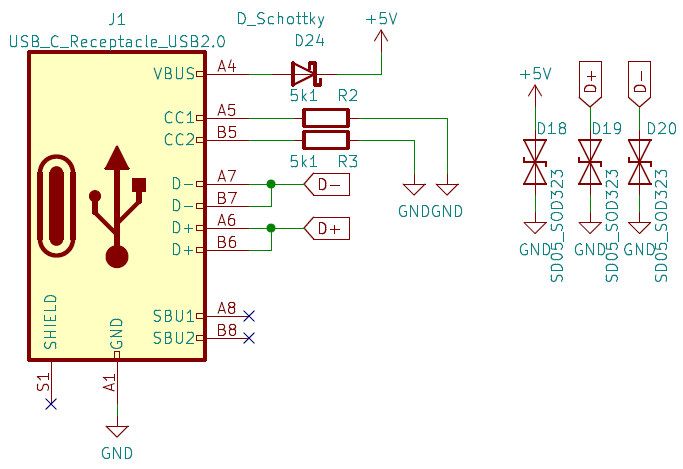
\includegraphics[scale=0.6]{obrazky/USB_C.png}
  \end{center}
  \caption[Zapojení konektoru USB-C]{Zapojení konektoru USB-C.}
\end{figure}

\begin{figure}[!h]
  \begin{center}
    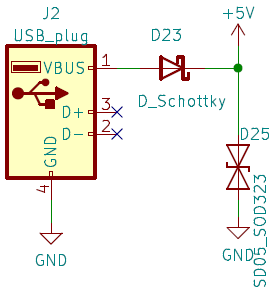
\includegraphics[scale=0.8]{obrazky/USB_A.png}
  \end{center}
  \caption[Zapojení konektoru USB-A]{Zapojení konektoru USB-A.}
\end{figure}


%o transilech k USB + Shotkyny (celkový odběr zařízení z USB - shotkyny na správný proud)
%o rezistorech 5,1k

%ke každé komponentě napsat odběr

%na konci bude muset být blokové schéma konkrétních (vybraných) modulů

%power led pro první prototyp, potom nebudou, kvůli šetření energie, protože je to na baterky a mohlo by to při hrách hráče mást

%zvukova sinalizace - piezo







\chapter{Návrh DPS}
%kulatá DPS - proč?

\section{Kapacitní tlačítka} 
Byl požadavek na 5 tlačítek. Jedno tlačítko je uprostřed a slouží jako hlavní tlačítko. U her bude používáno např. jako registrace průchodu místem apod. Bude tedy nejčastěji
používáno a zároveň může být stisknuto, když hráč běží, takže by mělo být co nejjednodušeji stisknutelné. Proto bylo navrženo větší než zbylá tlačítka. Konkrétně má 
5~$\times$~5~cm. Ostatní tlačítka slouží například jako směrovky, nebo pro vyklikávání nějakého kódu, aby získali nějakou informaci. Slouží tedy primárně, když účastník 
u sebaforu stojí, nebo sedí, a vyklikává. Díky tomu mohou být tlačítka menší než hlavní tlačítko, konkrétně mají 2~$\times$~2~cm. Tato tlačítka jsou proto umístěna 
po stranách hlavního tlačítka a jsou popsána BTN\_ENTER, BTN\_UP, BTN\_DOWN, BTN\_RIGHT a BTN\_LEFT.

\section{LED}
%do sekce o DPS se zmínit o jejich umístění - kruh, hodiny, proto 12 ks. (lze také rozdělit na 3 segmenty)

\section{Konektory}
%konektor USB C
%konektor USB A
%na kraji DPS